% !TEX program = xelatex
\documentclass[UTF8,fontset=fandol,a4paper,11pt]{ctexart}
\usepackage[margin=21mm,top=23mm,bottom=22mm,headheight=16pt]{geometry}
\usepackage{amsmath,amssymb,mathtools,bm}
\usepackage{tikz}
\usetikzlibrary{arrows.meta,calc,angles,quotes,patterns}
\usepackage{xcolor,booktabs,array,longtable,enumitem,fancyhdr,needspace}
\usepackage[unicode,hidelinks]{hyperref}
\definecolor{ink}{HTML}{24343C}
\definecolor{accent}{HTML}{166A70}
\definecolor{muted}{HTML}{65747A}
\definecolor{rulegray}{HTML}{D4DDE0}
\definecolor{warm}{HTML}{966037}
\color{ink}
\setlength{\parindent}{2em}
\setlength{\parskip}{4pt}
\linespread{1.12}
\AtBeginDocument{\setlength{\abovedisplayskip}{6pt plus 2pt minus 1pt}
\setlength{\belowdisplayskip}{6pt plus 2pt minus 1pt}
\setlength{\abovedisplayshortskip}{0pt plus 1pt}
\setlength{\belowdisplayshortskip}{4pt plus 1pt}}
\setlist[enumerate]{label=(\arabic*),leftmargin=2.3em,itemsep=3pt,topsep=4pt}
\setlist[itemize]{leftmargin=2em,itemsep=2pt,topsep=4pt}
\allowdisplaybreaks[1]
\setlength{\emergencystretch}{2em}
\setcounter{secnumdepth}{0}
\providecommand{\tightlist}{\setlength{\itemsep}{0pt}\setlength{\parskip}{0pt}}
\ctexset{section={format=\Large\bfseries\color{accent},beforeskip=10pt,afterskip=9pt},
subsection={format=\normalsize\bfseries\color{accent},beforeskip=10pt,afterskip=4pt},
subsubsection={format=\normalsize\bfseries,beforeskip=8pt,afterskip=3pt}}
\pagestyle{fancy}
\fancyhf{}
\fancyhead[L]{\small\color{muted}物理学难题集萃}
% 页眉仅保留书名；版本名称只在封面显示。
\fancyfoot[L]{\small\color{muted}\chapterlabel}
\fancyfoot[R]{\small\thepage}
\renewcommand{\headrulewidth}{0.4pt}
\renewcommand{\footrulewidth}{0pt}
\newcommand{\dd}{\mathop{}\!\mathrm{d}}
\newcommand{\vect}[1]{\bm{#1}}
\newcommand{\tagline}[1]{\noindent{\small\color{muted}#1}\par}
\newcommand{\result}[1]{\begin{equation*}\boxed{#1}\end{equation*}}
\newcommand{\figcaption}[1]{\par\vspace{2pt}{\small\color{muted}#1}\par}
\newcommand{\teach}[2]{\Needspace{4\baselineskip}\subsection*{讲解要点与追问}#1\par\smallskip\noindent\textbf{追问：}#2\par}
\newcommand{\workarea}{\par\vspace{7mm}\noindent{\small\color{muted}作答区}\par\vspace{4mm}
\noindent\textcolor{rulegray}{\rule{\linewidth}{0.3pt}}\par\vspace{16mm}
\noindent\textcolor{rulegray}{\rule{\linewidth}{0.3pt}}\par\vspace{16mm}
\noindent\textcolor{rulegray}{\rule{\linewidth}{0.3pt}}\par\vspace{16mm}
\noindent\textcolor{rulegray}{\rule{\linewidth}{0.3pt}}}
\tikzset{axis/.style={-{Stealth[length=2mm]},thin,color=muted},
motion/.style={-{Stealth[length=2.3mm]},thick,color=accent},
force/.style={-{Stealth[length=2.3mm]},thick,color=warm},
traj/.style={thick,color=accent},guide/.style={dashed,thin,color=muted},
object/.style={thick,color=ink},every node/.style={font=\small}}\widowpenalty=10000\clubpenalty=10000\displaywidowpenalty=10000\newcommand{\chapterlabel}{综合试题（三）}







\hypersetup{pdftitle={综合试题（三）·学生版},pdfauthor={}}

\begin{document}\pdfbookmark[0]{综合试题（三）}{cover}

\thispagestyle{empty}\vspace*{22mm}

\noindent{\Huge\bfseries 物理学难题集萃}\par\vspace{12mm}

\noindent{\LARGE 综合试题（三）}\par\vspace{12mm}

\noindent{\Large\color{accent}学生版}\par\vspace{9mm}

\noindent\textcolor{accent}{\rule{\linewidth}{1pt}}\par\vspace{9mm}

\noindent 第1--6题\par\vfill\clearpage

\pdfbookmark[1]{题目目录}{contents}\section*{题目目录}

\begin{longtable}{@{}r p{113mm} r@{}}\toprule 题号 & 题目 & 页码\\\midrule

\hyperref[q:1]{1} & \hyperref[q:1]{滚轮线的加速度、曲率与等时摆} & \pageref{q:1} \\

\hyperref[q:2]{2} & \hyperref[q:2]{限定地面投影范围的卫星轨道} & \pageref{q:2} \\

\hyperref[q:3]{3} & \hyperref[q:3]{悬挂弹性杆的长度与密度} & \pageref{q:3} \\

\hyperref[q:4]{4} & \hyperref[q:4]{阻尼振动、感应制动与受迫响应} & \pageref{q:4} \\

\hyperref[q:5]{5} & \hyperref[q:5]{随机选择、方向分布与二维分子速率} & \pageref{q:5} \\

\hyperref[q:6]{6} & \hyperref[q:6]{四相电源与断线后的浮动星点} & \pageref{q:6} \\

\bottomrule\end{longtable}

\clearpage

\pdfbookmark[2]{第 1 题 滚轮线的加速度、曲率与等时摆}{q1}

\section*{第 1 题\quad 滚轮线的加速度、曲率与等时摆}\label{q:1}


\begin{enumerate}
\item 半径$R$的圆环在水平地面向前纯滚动，环心速率恒为$v_0>0$。求环上任一点$P$在一周内加速度大小最大值与最小值之差。
\item 无论环心匀速还是变速前进，只要始终向前纯滚动，环上一点的轨迹都是同一条滚轮线。求轨迹最低接地点的曲率半径极限$\rho_1$及最高点的曲率半径$\rho_2$，并解释最低点为何需用极限表述。
\item 将生成圆环置于水平$x$轴下方沿轴纯滚动，得到向下凹的摆线轨道。小球从该轨道一拱内的任一光滑、非最低位置静止释放，无摩擦往返。已知其周期与质量及初位置无关，求全周期$T$，并由弧长坐标推导这种等时性。
\end{enumerate}
重力加速度为$g$；配图中区分向上滚轮线的接地尖点与下方凹轨道的光滑稳定最低点。


\begin{center}\begin{minipage}{.98\linewidth}\centering
\begin{tikzpicture}[scale=.85,transform shape]

\draw[axis] (-.4,0)--(5.7,0) node[right] {$x$};
\draw[object] (0,.8) circle (.8);
\fill (0,.8) circle (2pt) node[left] {$C$};
\draw[motion] (0,.8)--(1.2,.8) node[right] {$v_0$};
\fill (0,0) circle (2pt) node[below] {$P$};
\node at (2.6,2.3) {向上生成：接地处为尖点};
\draw[traj,domain=0:360,samples=160] plot ({.8*(rad(\x)-sin(\x))},{1*.8*(1-cos(\x))});
\begin{scope}[yshift=-2cm]
\draw[axis] (-.4,0)--(5.7,0);\draw[traj,domain=0:360,samples=160] plot ({.8*(rad(\x)-sin(\x))},{-1*.8*(1-cos(\x))});
\fill (2.513,-1.6) circle (2pt) node[below] {稳定最低点};
\node at (2.6,-2.4) {倒置凹轨道：最低点光滑};
\end{scope}

\end{tikzpicture}
\figcaption{图综三.1\quad 同一摆线的两种朝向；等时摆沿下方凹轨道运动。}
\end{minipage}\end{center}

\par\vspace{5mm}\noindent{\small\color{muted}作答区}\par\vspace{3mm}\noindent\textcolor{rulegray}{\rule{\linewidth}{0.3pt}}\par\vspace{12mm}\noindent\textcolor{rulegray}{\rule{\linewidth}{0.3pt}}

\clearpage

\pdfbookmark[2]{第 2 题 限定地面投影范围的卫星轨道}{q2}

\section*{第 2 题\quad 限定地面投影范围的卫星轨道}\label{q:2}


在一个假想规则下，卫星与地心连线同地表的交点必须始终位于本国领土或领海。忽略摄动，地球视为球形。取地球自转周期$T_0=1\,\mathrm d=86400\,\mathrm s$，同步圆轨道的地心距离$R_0=4.21\times10^4\,\mathrm{km}$。
\begin{enumerate}
\item 一个国家仅有北纬$20^\circ$至$50^\circ$的领土，能否发射入轨后不靠动力且始终不越界的卫星？另一个国家有北纬$15^\circ$至南纬$10^\circ$的领土，且有赤道领土，能否找到一种可行轨道？
\item 某国在赤道只拥有总经度宽$\theta_0=2^\circ$的连续区域，发射周期$T_0$的赤道面无动力椭圆轨道卫星。长短半轴为$A,B$，焦距$C=\sqrt{A^2-B^2}$，偏心率$e=C/A\ll1$。求使卫星地面投影不越出该经度范围的最大$e$，保留一阶推导，并说明全摆幅与半摆幅。
\item 另有卫星需靠动力定点在北纬$\phi=40^\circ$的某城市上空，距地心恰为$R_0$。入轨后卫星主体质量100公斤，火箭空载1000公斤，燃料9000公斤；喷气相对速度$u=5\,\mathrm{km/s}$。求维持该位置的最久时间，给出所需推力方向和随质量变化的燃耗关系。
\end{enumerate}
第（2）问可选择初始经度使投影摆动区间居中；第（3）问假定推力连续可调，忽略其他燃耗。


\begin{center}\begin{minipage}{.98\linewidth}\centering
\begin{tikzpicture}[scale=.8,transform shape]

\draw[object] (0,0) circle (1.7);
\draw[guide] (-2,0)--(2,0) node[right] {赤道};
\draw[guide] (0,-2.1)--(0,2.1) node[above] {地轴};
\draw[traj] (-1.597477455,0.581434244)--(1.597477455,0.581434244);
\draw[traj] (-1.092738936,1.302275553)--(1.092738936,1.302275553);
\node[right] at (1.7,1) {$20^\circ$至$50^\circ$};
\begin{scope}[xshift=6.5cm]
\draw[object] (0,0) circle (1.1);
\draw[guide] (0,-1.7)--(0,2.3) node[above] {$z$};
\draw[guide] (-1.5,0)--(2.8,0);
\fill (2.1,1.76) circle (3pt) node[above right] {动力定点};
\draw[object] (0,0)--(2.1,1.76) node[midway,above left] {$R_0$};
\draw[guide] (.8,0) arc[start angle=0,end angle=40,radius=.8];
\node at (1.05,.35) {$\phi$};
\end{scope}

\end{tikzpicture}
\figcaption{图综三.2\quad 不含赤道的纬带与固定北纬位置；距离均由地心量起。}
\end{minipage}\end{center}

\par\vspace{5mm}\noindent{\small\color{muted}作答区}\par\vspace{3mm}\noindent\textcolor{rulegray}{\rule{\linewidth}{0.3pt}}\par\vspace{12mm}\noindent\textcolor{rulegray}{\rule{\linewidth}{0.3pt}}

\clearpage

\pdfbookmark[2]{第 3 题 悬挂弹性杆的长度与密度}{q3}

\section*{第 3 题\quad 悬挂弹性杆的长度与密度}\label{q:3}


一根均匀弹性圆柱杆的自然长度为$L_0$、质量为$m$，忽略形变引起的截面积变化。将整根杆沿轴线均匀拉伸时，其劲度系数为$K$，并假定在所讨论范围内服从胡克定律。现将上端固定，杆在重力作用下竖直悬挂，达到静止。

（1）求杆的伸长量。（2）特别取$K=mg/L_0$，求悬挂后质量线密度随到上端距离$x$的分布，并写明$x$的范围。须区分形变前的材料坐标与形变后的空间坐标。


\begin{center}\begin{minipage}{.98\linewidth}\centering
\begin{tikzpicture}[scale=.85,transform shape]

\fill[accent!15] (0,0) rectangle (.7,-3);
\draw[object] (0,0) rectangle (.7,-3);
\fill[warm!25] (0,-.6) rectangle (.7,-.9);
\draw[axis,<->] (-.6,0)--(-.6,-3) node[midway,left] {$L_0$};
\node at (.35,.5) {自然状态};
\begin{scope}[xshift=4cm]
\draw[object] (-.5,0)--(1.2,0);
\fill[accent!15] (0,0) rectangle (.7,-4.5);
\draw[object] (0,0) rectangle (.7,-4.5);
\fill[warm!25] (0,-1.14) rectangle (.7,-1.665);
\draw[axis,<->] (1.3,0)--(1.3,-4.5) node[midway,right] {$L_0+\Delta L$};
\draw[axis] (2.7,0)--(2.7,-4.8) node[below] {$x$向下};
\node at (.35,.5) {悬挂状态};
\end{scope}
\draw[guide,->] (.8,-.75)--(3.9,-1.4);

\end{tikzpicture}
\figcaption{图综三.3\quad 同色小段含相同材料质量，悬挂后长度和空间位置均改变。}
\end{minipage}\end{center}

\par\vspace{5mm}\noindent{\small\color{muted}作答区}\par\vspace{3mm}\noindent\textcolor{rulegray}{\rule{\linewidth}{0.3pt}}\par\vspace{12mm}\noindent\textcolor{rulegray}{\rule{\linewidth}{0.3pt}}

\clearpage

\pdfbookmark[2]{第 4 题 阻尼振动、感应制动与受迫响应}{q4}

\section*{第 4 题\quad 阻尼振动、感应制动与受迫响应}\label{q:4}


（1）分别建立下列系统的运动方程，讨论能否振动及其条件。

甲：质量$m$、密度为水的$a$倍（$a>1$）的小球，用长$l$的轻质刚杆悬于水中，水对球的阻力为$-\gamma\boldsymbol v$。忽略杆的浮力、阻力，讨论小角度运动。

乙：间距$l$的水平平行导轨上有质量$m$的导体棒，与电阻$R$、自感$L$串联构成闭合回路。匀强磁场$B$垂直纸面向里。导轨和棒的电阻、摩擦忽略；初始棒向右以$v_0$运动，回路电流为零。分析速度和电流随时间的变化。

（2）对一般受迫振动方程
\[
\ddot x+2\beta\dot x+\omega_0^2x=h\cos pt
\]
（$\beta,\omega_0,h,p>0$），求完整解的结构和稳态振幅、相位，并说明暂态何时消失、振幅在何种频率达到最大。


\begin{center}\begin{minipage}{.98\linewidth}\centering
\begin{tikzpicture}[scale=.65,transform shape]

\draw[object] (-.7,0)--(.7,0);
\draw[guide] (0,0)--(0,-3.1);
\draw[object] (0,0)--(1.4,-2.4) node[midway,right] {$l$};
\fill[accent] (1.4,-2.4) circle (5pt) node[right] {$m$};
\draw[guide] (0,-.9) arc[start angle=-90,end angle=-59.74,radius=.9];
\node at (.45,-1.15) {$\theta$};
\draw[guide] (-1.5,-.8)--(2.7,-.8) node[right] {水面};

\begin{scope}[xshift=5.8cm]
\draw[object] (0,0)--(0,2)--(1.1,2);
\draw[object] (2.5,2)--(4,2)--(4,0)--(0,0);
\draw[object] (1.1,1.8) rectangle (2.5,2.2);
\node[above] at (1.8,2.2) {$L$};
\fill[white] (-.2,.5) rectangle (.2,1.5);
\draw[object] (-.2,.5) rectangle (.2,1.5);
\node[left] at (-.2,1) {$R$};
\draw[object,line width=2pt] (4,0)--(4,2);
\draw[motion] (4.2,1.3)--(5.3,1.3) node[right] {$v$};
\draw[motion] (3.7,.4)--(3.7,1.3) node[left] {$i$};
\node at (2,1) {$\otimes B$};
\draw[axis,<->] (5.8,0)--(5.8,2) node[midway,right] {$l$};
\end{scope}

\end{tikzpicture}
\figcaption{图综三.4\quad 水中轻杆摆与含串联电阻、自感的导体棒回路。}
\end{minipage}\end{center}

\par\vspace{5mm}\noindent{\small\color{muted}作答区}\par\vspace{3mm}\noindent\textcolor{rulegray}{\rule{\linewidth}{0.3pt}}\par\vspace{12mm}\noindent\textcolor{rulegray}{\rule{\linewidth}{0.3pt}}

\clearpage

\pdfbookmark[2]{第 5 题 随机选择、方向分布与二维分子速率}{q5}

\section*{第 5 题\quad 随机选择、方向分布与二维分子速率}\label{q:5}


（1）一位成人把糖放在左右手之一，小孩猜中即可得到糖。成人可以根据此前的结果改变藏糖方法，但每次必须先固定藏糖的手，再让小孩猜。小孩怎样随机选择，才能使每次猜中的概率不受藏糖策略影响？连续猜$N$次，所得糖数的期望和方差是多少？

（2）在平面上，点$S$与水平直线的垂直距离为$h$，垂足为$O$。从$S$向该直线发出一条随机射线，与向下垂线的夹角$\theta$在$(-\pi/2,\pi/2)$均匀分布。求落点相对$O$的有向坐标$x$的概率密度。

（3）二维理想气体中，分子质量为$m$，温度为$T$。两个正交速度分量独立，均服从均值为零、方差为$k_{\rm B}T/m$的高斯分布。求二维速率分布，进而求最概然速率、平均速率和方均根速率。玻尔兹曼常量记为$k_{\rm B}$。


\begin{center}\begin{minipage}{.98\linewidth}\centering
\begin{tikzpicture}[scale=.73,transform shape]

\node at (0,2) {成人先固定藏糖手};
\node[draw,rounded corners] (H) at (0,1) {孩子独立抛公平硬币};
\node[draw] (L) at (-1,-.2) {猜左};
\node[draw] (R) at (1,-.2) {猜右};
\draw[->] (H)--(L) node[midway,left] {$1/2$};
\draw[->] (H)--(R) node[midway,right] {$1/2$};
\begin{scope}[xshift=4cm]
\draw[axis] (-1.3,0)--(1.8,0) node[right] {$x$};
\fill (0,2) circle (2pt) node[above] {$S$};
\draw[guide] (0,2)--(0,0) node[below] {$O$};
\draw[object] (0,2)--(1.3,0);
\node[left] at (0,1) {$h$};
\end{scope}
\begin{scope}[xshift=8.5cm]
\draw[axis] (-1.4,0)--(1.6,0) node[right] {$v_x$};
\draw[axis] (0,-1.3)--(0,1.6) node[above] {$v_y$};
\draw[object] (0,0) circle (1);
\draw[guide] (0,0)--(.707,.707) node[midway,above left] {$v$};
\end{scope}

\end{tikzpicture}
\figcaption{图综三.5\quad 藏糖猜测、随机方向落点与二维速度平面的三个概率模型。}
\end{minipage}\end{center}

\par\vspace{5mm}\noindent{\small\color{muted}作答区}\par\vspace{3mm}\noindent\textcolor{rulegray}{\rule{\linewidth}{0.3pt}}\par\vspace{12mm}\noindent\textcolor{rulegray}{\rule{\linewidth}{0.3pt}}

\clearpage

\pdfbookmark[2]{第 6 题 四相电源与断线后的浮动星点}{q6}

\section*{第 6 题\quad 四相电源与断线后的浮动星点}\label{q:6}


四相电源的中性点为$N$，各相端点依次为$A,B,C,D$。对$N$的电势为
\[
E_1=E_0\cos\omega t,\quad E_2=E_0\cos(\omega t+\pi/2),\quad
E_3=E_0\cos(\omega t+\pi),\quad E_4=E_0\cos(\omega t+3\pi/2).
\]
四个负载$Z_A,Z_B,Z_C,Z_D$接成星形，星点为$O$。图中$x$是$N$与$O$间的中性线，$y$是$D$相引线；各相电流正方向均由相端流向$O$。

（1）求$U_{AB},U_{AC},U_{AD}$的瞬时表达式。若各相电压有效值为$220\,\mathrm V$，求这三个线电压的峰值。

（2）现同时断开$x,y$，用$Z_A,Z_B,Z_C$和电源电势的复振幅求$A$相电流；须列出所用基尔霍夫方程。

（3）断线情形下取$Z_A=R$、$Z_B=j\omega L$、$Z_C=1/(j\omega C)$，其中$L=R/\omega$、$C=1/(\omega R)$。求$A$相电流的振幅和相位，并求出其余两相电流和各相平均功率。负载与电源均为理想元件，采用$\Re(\widetilde E e^{j\omega t})$约定。


\begin{center}\begin{minipage}{.98\linewidth}\centering
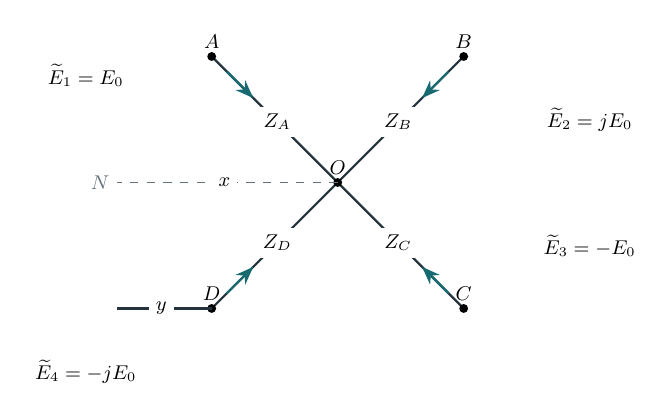
\begin{tikzpicture}[scale=.8,transform shape]

\coordinate (A) at (-2,2);\coordinate (B) at (2,2);
\coordinate (C) at (2,-2);\coordinate (D) at (-2,-2);
\coordinate (O) at (0,0);
\foreach \p/\z in {A/A,B/B,C/C,D/D}{
\draw[object] (\p)--(O);
\node[fill=white,inner sep=3pt] at ($(\p)!.52!(O)$) {$Z_\z$};
\fill (\p) circle (2pt) node[above] {$\p$};
}
\fill (O) circle (2pt) node[above] {$O$};
\foreach \p in {A,B,C,D}{\draw[motion] ($(\p)!.12!(O)$)--($(\p)!.33!(O)$);}

\draw[guide] (0,0)--(-3.5,0) node[left] {$N$};
\node[fill=white] at (-1.8,0) {$x$};
\draw[object] (-2,-2)--(-3.5,-2);
\node[fill=white] at (-2.8,-2) {$y$};
\node at (4,1) {$\widetilde E_2=jE_0$};
\node at (4,-1) {$\widetilde E_3=-E_0$};
\node at (-4,1.7) {$\widetilde E_1=E_0$};
\node at (-4,-3) {$\widetilde E_4=-jE_0$};

\end{tikzpicture}
\figcaption{图综三.6\quad 四相星形负载；$x$为中性线，$y$为$D$相引线。}
\end{minipage}\end{center}

\par\vspace{5mm}\noindent{\small\color{muted}作答区}\par\vspace{3mm}\noindent\textcolor{rulegray}{\rule{\linewidth}{0.3pt}}\par\vspace{12mm}\noindent\textcolor{rulegray}{\rule{\linewidth}{0.3pt}}

\end{document}
